\section{Empirical Performance Analysis}
\label{fairness_justicia_sec:experiments}
In this section, we discuss the empirical studies to evaluate the performance of {\justicia} in verifying different fairness metrics. We first discuss the experimental setup and the objective of the experiments and then evaluate the experimental results.
\subsection{Experimental Setup}
We have implemented a prototype of {\justicia} in Python (version $ 3.7.3 $). The core computation of {\justicia} relies on solving SSAT formulas using an off-the-shelf SSAT solver. To this end, we employ the state of the art RE-SSAT solver of~\cite{lee2017solving} and the ER-SSAT solver of~\cite{lee2018solving}. Both solvers output the exact  satisfying probability of the SSAT formula. 

For comparative evaluation of {\justicia}, we have experimented with two state-of-the-art distributional verifiers FairSquare and VeriFair, and also a sample-based fairness measuring tool: AIF360. In the experiments, we have studied three type of classifiers: decision tree, logistic regression classifier, and CNF learner. Decision tree and logistic regression are implemented using scikit-learn module of Python~\cite{PVGMTGB2011} and we use the MaxSAT-based CNF learner, namely IMLI~\cite{GM2019}. We have used the PySAT library~\cite{imms-sat18} for encoding the decision function of the logistic regression classifier into a CNF formula. In our experiments, we have verified two fairness-enhancing algorithms: reweighing algorithm~\cite{kamiran2012data} and optimized pre-processing  algorithm~\cite{calmon2017optimized}. 
We have experimented on multiple datasets containing multiple sensitive features: the UCI\footnote{\url{ http://archive.ics.uci.edu/ml}} Adult and German-credit dataset,  ProPublica’s COMPAS recidivism dataset~\cite{angwin2016machine}, Ricci dataset~\cite{mcginley2010ricci}, and Titanic dataset\footnote{\url{https://www.kaggle.com/c/titanic}}.
\iffalse 
Since both {\justicia}  and FairSquare take a  probability distribution of the features as input, we perform five-fold cross validation, use the train set for learning the classifier, compute distribution on the test set and finally verify fairness metrics such as disparate impact and statistical parity difference on the distribution. 
\fi
%that pre-process the dataset to mitigate its bias

Our empirical studies have following objectives:

\begin{enumerate}
	\item How accurate and scalable {\justicia} is with respect to existing fairness verifiers: FairSquare and VeriFair?
	\item Can {\justicia} verify the effectiveness of different fairness-enhancing algorithms on different datasets?
	\item Can {\justicia} verify fairness in the presence of compound sensitive groups?
	\item How robust is {\justicia} in comparison to sample-based tools like AIF360 for varying sample sizes?
	\item How do the computational efficiencies of {\justicialearn} and {\justiciaenum} compare?
\end{enumerate}


%\begin{enumerate}
%	\item How accurate and scalable {\justicia} is with respect to existing fairness verifiers, FairSquare and VeriFair?
%	\item Can {\justicia} verify the effectiveness of different fairness-enhancing algorithms on different datasets?
%	\item Can {\justicia} verify fairness in the presence of compound sensitive groups?
%	\item How robust is {\justicia} in comparison to empirical tools like AIF360 for varying sample sizes?
%\end{enumerate}

Our experimental studies validate that {\justicia} is more accurate and scalable than the state-of-the-art verifiers: FairSquare and VeriFair. {\justicia} is able to verify the effectiveness of different fairness-enhancing algorithms for multiple fairness metrics and datasets. {\justicia} achieves scalable performance in the presence of compound sensitive groups that the existing verifiers cannot handle.  {\justicia} is also more robust than the sample-based tools such as AIF360.
Finally, {\justicialearn} is significantly efficient in terms of runtime than {\justiciaenum}.


\subsection{Experimental Analysis}



\begin{table}[t!]
    \centering
%        \vspace*{-.2em}
        \setlength{\tabcolsep}{.1em}
            \begin{tabular}{ccccccc}
                \toprule
                Metric & Exact  & {\justicia} & FairSquare & VeriFair & AIF360\\
                 \midrule
				Disparate impact &  $ 0.26 $  &  $ 0.25 $    &  $ 0.99 $  &  $ 0.99 $  &  $ 0.25 $  \\
				Stat. parity &  $ 0.53 $  &  $ 0.54 $    & \textemdash & \textemdash &  $ 0.54 $  \\
                \bottomrule
    \end{tabular}
 \caption{Results on synthetic benchmark.  `\textemdash'~ refers that the verifier cannot compute the metric. }
\label{fairness_justicia_tab:synthetic}
\end{table}


%\subsubsection{Performance of Different Verifiers.}
\subsubsection{Accuracy: Less Than $  1\%$-error} 
In order to assess the accuracy of different verifiers, we have considered the decision tree in Figure~\ref{fairness_justicia_fig:fair_example} for which the fairness metrics  are analytically computable. 
In Table~\ref{fairness_justicia_tab:synthetic}, we show the computed fairness metrics by {\justicia}, FairSquare, VeriFair, and AIF360. We observe that {\justicia} and AIF360  yield more accurate estimates of DI and SP compared against the ground truth values of fairness metrics with less than $1\%$ error. In contrast, FairSquare and VeriFair  estimate DI to be $0.99$ and thus, being unable to verify the fairness violation. Therefore, {\justicia} is significantly more accurate than the existing formal verifiers: FairSquare and VeriFair. 
%First we observe that both RE and ER encoding result in the same disparate impact, thereby showing the equivalence between the two encodings.  


\begin{comment}
\begin{table}[h]
 \caption[Scalability of {\justicia}]{Scalability of different verifiers in terms of execution time (in seconds).  DT and LR refer to decision tree and logistic regression classifier, respectively. `\textemdash'~ refers to timeout.}
 \label{fairness_justicia_tab:FS_VF_Justicia}
 
    \centering
%        \setlength{\tabcolsep}{.3em}
%        \vspace*{-.3em}
            \begin{tabular}{lrrrrrrrr}
                \toprule
                Dataset   & \multicolumn{2}{c}{Ricci} & \multicolumn{2}{c}{Titanic} & \multicolumn{2}{c}{COMPAS} &  \multicolumn{2}{c}{Adult} \\ 
                \cmidrule(lr){2-3}
                \cmidrule(lr){4-5}
                \cmidrule(lr){6-7}
                \cmidrule(lr){8-9}
                

                Classifier & DT     & LR  & DT & LR  & DT  & LR  & DT  & LR \\ \midrule


{\justicia} &  $ 0.1  $  &  $ 0.2  $  &  $ 0.1  $  &  $ 0.9  $  &  $ 0.1  $  &  $ 0.2  $  &  $ 0.2  $  &  $ 1.0  $  \\
FairSquare &  $ 4.8  $  & \textemdash &  $ 16.0  $  & \textemdash &  $ 36.9  $  & \textemdash & \textemdash & \textemdash \\
VeriFair &  $ 5.3  $  &  $ 2.2  $  &  $ 1.2  $  &  $ 0.8  $  &  $ 15.9  $  &  $ 11.3  $  &  $ 295.6  $  &  $ 61.1  $  \\
                \bottomrule
    \end{tabular}
%\vspace*{-1em}
\end{table}


\begin{table}[h]
	\centering
	\begin{tabular}{lrrrrrrrr}
		\toprule
		Dataset & Classifier & FairSquare & VeriFair & {\justicia} \\
		\midrule
		\multirow{2}{*}{Ricci} & Decision Tree & $ 4.8 $ & $ 5.3 $ & $ \mathbf{0.1} $ \\
		 & Logistic Regression & \textemdash & $ 2.2 $ & $ \mathbf{0.2} $ \\
		\multirow{2}{*}{Titanic} & Decision Tree & $ 16 $ & $ 1.2 $ & $ \mathbf{0.1} $ \\
		& Logistic Regression & \textemdash & $ \textbf{0.8} $ & $ 0.9 $ \\
		\multirow{2}{*}{COMPAS} & Decision Tree & $ 36.9 $ & $ 15.9 $ & $ \mathbf{0.1} $ \\
		& Logistic Regression & \textemdash & $ 11.3 $ & $ \mathbf{0.2} $ \\
		\multirow{2}{*}{Adult} & Decision Tree & \textemdash & $ 295.6 $ & $ \mathbf{0.2} $ \\
		& Logistic Regression & \textemdash & $ 61.1 $ & $ \mathbf{1.0} $ \\
		\bottomrule
	\end{tabular}
\end{table}
\end{comment}


\begin{table}[!t]
	\caption[Scalability of {\justicia}]{Scalability of different verifiers in terms of execution time (in seconds). The number in bold refers to the best result incurring minimum execution time among competitive verifiers. `\textemdash'~ refers to timeout.}
	\label{fairness_justicia_tab:FS_VF_Justicia}
	\centering
	\begin{tabular}{lrrrrrrrr}
		\toprule
		Classifier & Dataset & FairSquare & VeriFair & {\justicia} \\
		\midrule
		\multirow{4}{*}{Decision Tree} & Ricci & $ 4.8 $ & $ 5.3 $ & $ \mathbf{0.1} $ \\
		& Titanic & $ 16 $ & $ 1.2 $ & $ \mathbf{0.1} $ \\
		& COMPAS & $ 36.9 $ & $ 15.9 $ & $ \mathbf{0.1} $ \\
		& Adult & \textemdash & $ 295.6 $ & $ \mathbf{0.2} $ \\
		\\
		\multirow{4}{*}{Logistic Regression} & Ricci & \textemdash & $ 2.2 $ & $ \mathbf{0.2} $ \\
		& Titanic & \textemdash & $ \textbf{0.8} $ & $ 0.9 $ \\
		& COMPAS & \textemdash & $ 11.3 $ & $ \mathbf{0.2} $ \\
		& Adult & \textemdash & $ 61.1 $ & $ \mathbf{1.0} $ \\
		
		\bottomrule
		
	\end{tabular}
\end{table}



\subsubsection{Scalability: $ 1 $ to $ 3 $ Orders of Magnitude Speed-up} 
%Since {\justicia} appears to be more accurate than FairSquare and VeriFair in the synthetic benchmark, 
We have tested the scalability of {\justicia}, FairSquare, and VeriFair on practical benchmarks with a timeout of $900$ seconds and reported the execution time of these verifiers on decision tree and logistic regression in Table~\ref{fairness_justicia_tab:FS_VF_Justicia}. We observe that {\justicia} shows impressive scalability than the competing verifiers. Particularly, {\justicia} is $ 1 $ to $ 2 $ orders of magnitude faster than FairSquare and  $ 1 $ to $ 3 $ orders of magnitude faster than VeriFair. Additionally, FairSquare times out in most  benchmarks.
Thus, {\justicia} is not only accurate but also scalable than the existing verifiers. 


\begin{figure*}
	\centering
	\subfloat{
		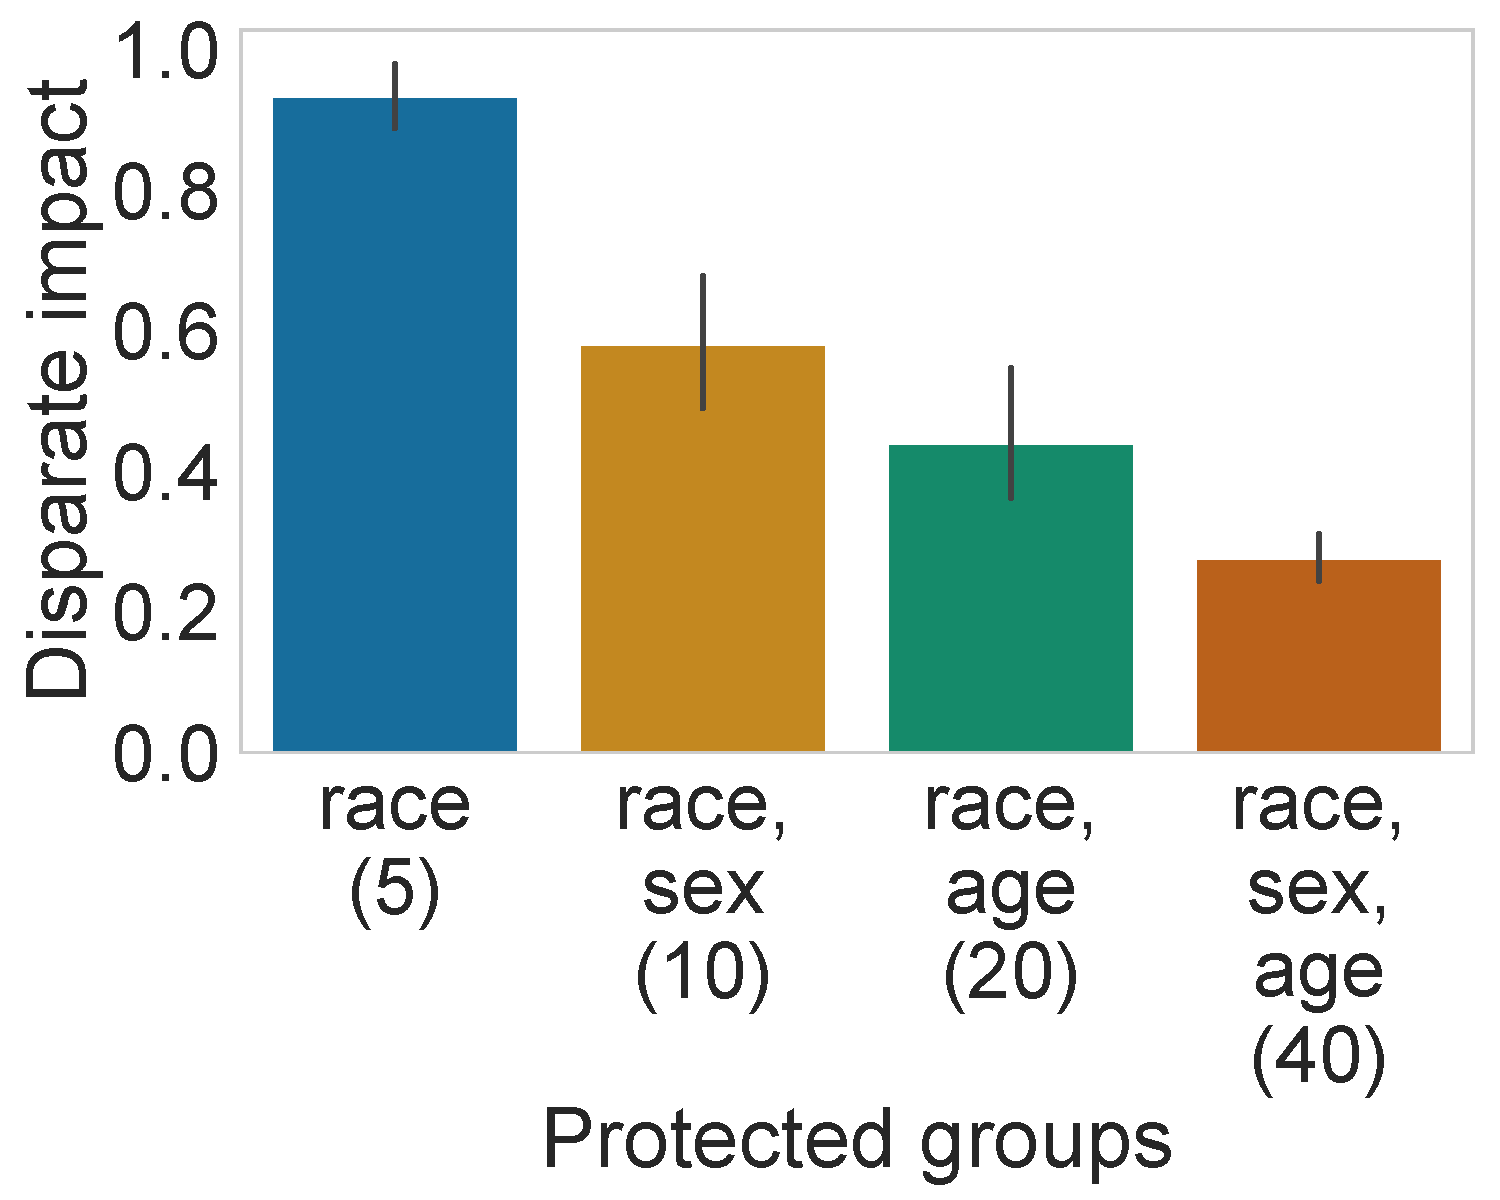
\includegraphics[scale=.2]{figures/fairness/justicia/sensitive_attribute_race_di_Adult_DT_RE.pdf}
	}
	\subfloat{
		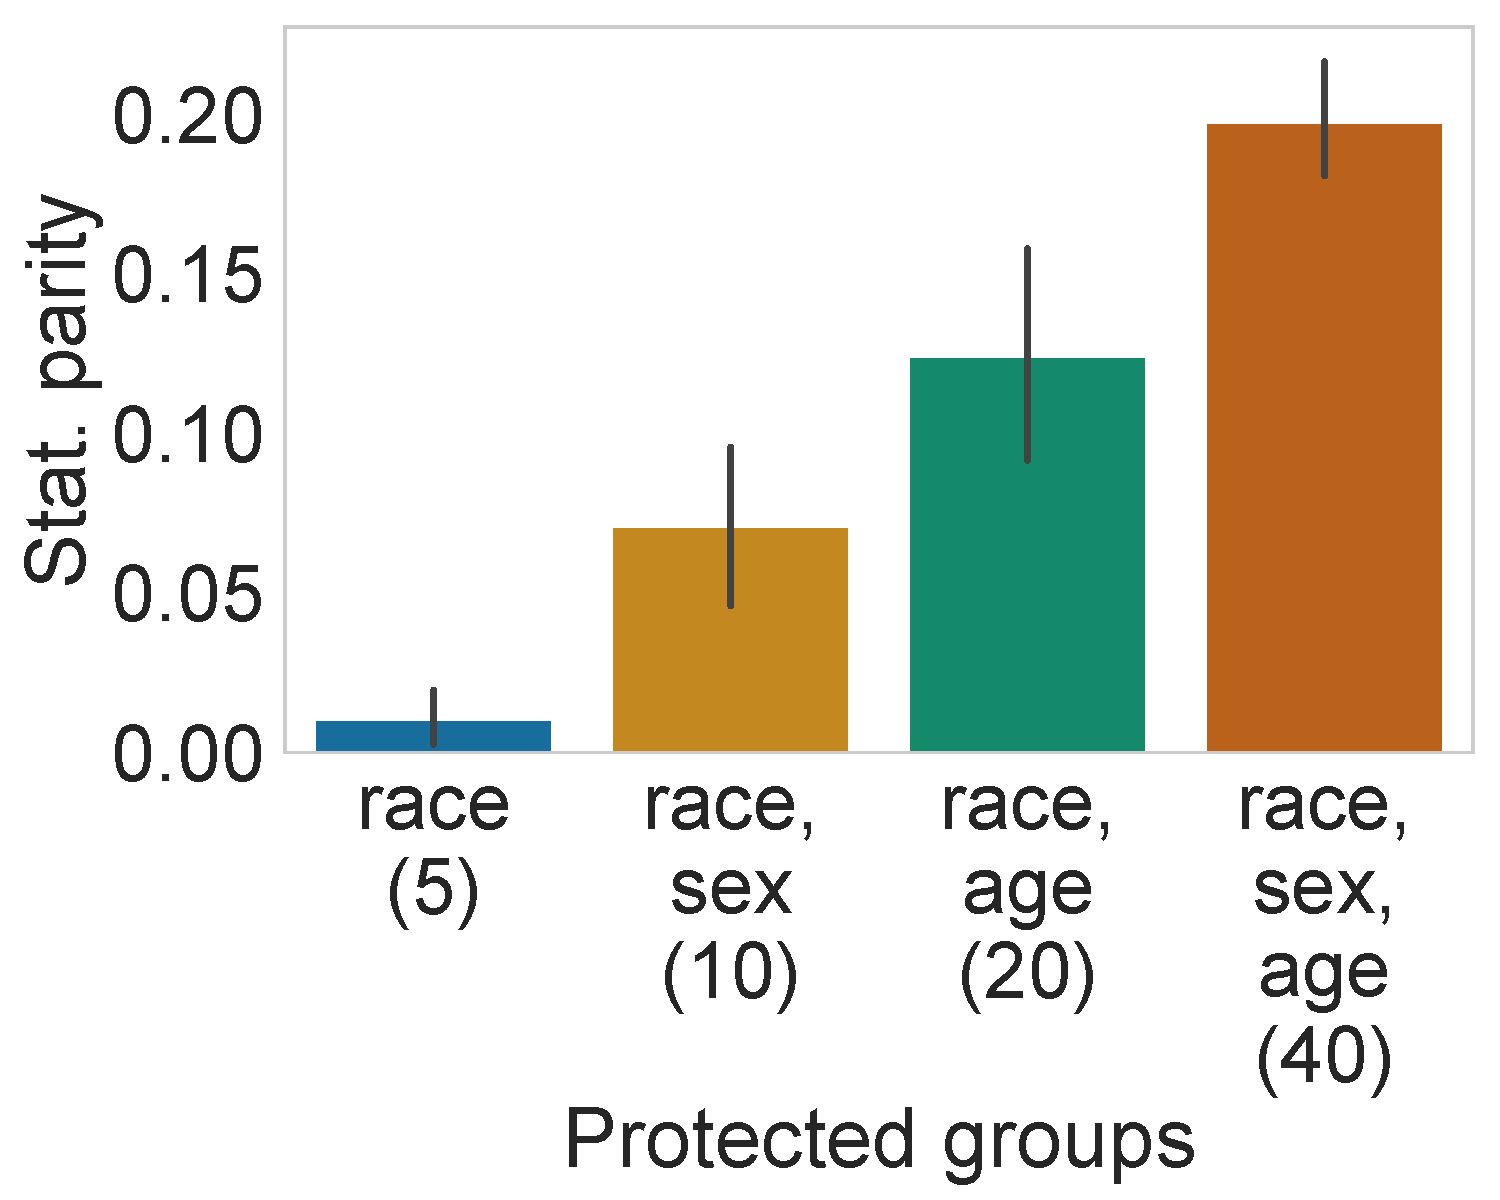
\includegraphics[scale=.2]{figures/fairness/justicia/sensitive_attribute_race_spd_Adult_DT_RE.pdf}
	}
	\caption[Fairness verification on compound sensitive groups]{Fairness metrics measured by {\justicia} for different sensitive groups in the Adult dataset. The number within parenthesis in the xticks denotes total compound groups.}
	\label{fairness_justicia_fig:sensitive_groups}
\end{figure*}



\subsubsection{Verification: Detecting Compounded Discrimination in Protected Groups.}
We have tested {\justicia} for datasets consisting of multiple sensitive features and reported results in Figure~\ref{fairness_justicia_fig:sensitive_groups}. {\justicia} operates on datasets with even 40 compound sensitive groups and can potentially scale more than that while the state-of-the-art fairness verifiers (e.g., FairSquare and VeriFair) consider a single sensitive feature with two sensitive groups. Thus, {\justicia} removes an important limitation in practical fairness verification, which was previously restricted to Boolean sensitive groups. Additionally, in most datasets, we observe that disparate impact decreases and thus, discrimination increases as more compound sensitive groups are considered. For instance, when we increase the total  groups from $ 5 $ to $ 40 $ in the Adult dataset, disparate impact decreases from around $ 0.9 $ to $ 0.3 $, thereby detecting higher discrimination. Thus, {\justicia} detects that the marginalized individuals of a specific type (e.g., `race')  are even more discriminated and marginalized when they also belong to a marginalized group of another type (e.g., `sex').


\begin{sidewaystable}
	\caption[Fairness verification of fairness metrics and algorithms]{Verification of different fairness enhancing algorithms for multiple datasets and classifiers using {\justicia}. Numbers in bold refer to fairness improvement  compared against the unprocessed (orig.) dataset. RW and OP refer to reweighing and optimized-preprocessing algorithm respectively. }\label{fairness_justicia_tab:fair_algo_verification}
	\footnotesize       
    \centering
%        \setlength{\tabcolsep}{.3em}
            \begin{tabular}{ll
            				ccc
            				ccc
%            				ccc
%            				ccc
            				ccc
            				ccc}
                \toprule
                \multirow{3}{*}{Classifier}& Dataset $ \rightarrow $   & 
                \multicolumn{6}{c}{Adult} &
%                \multicolumn{6}{c}{German} &
                \multicolumn{6}{c}{COMPAS} \\ 
                \cmidrule(lr){3-8}
                \cmidrule(lr){9-14}
%                \cmidrule(lr){15-20}
                & Sensitive  $ \rightarrow $ & 
                \multicolumn{3}{c}{Race}   & \multicolumn{3}{c}{Sex}  &
%                \multicolumn{3}{c}{Age}   & \multicolumn{3}{c}{Sex}  &
                \multicolumn{3}{c}{Race}   & \multicolumn{3}{c}{Sex}
                \\ 
                \cmidrule(lr){3-5}
                \cmidrule(lr){6-8}
                \cmidrule(lr){9-11}
                \cmidrule(lr){12-14}
%                \cmidrule(lr){15-17}
%                \cmidrule(lr){18-20}

                 & Algorithm  $ \rightarrow $ &  
                orig. & RW & OP & 
                orig. & RW & OP &
%                orig. & RW & OP &
%                orig. & RW & OP &
                orig. & RW & OP &
                orig. & RW & OP \\ 
                \midrule
          
              
              
              \multirow{3}{*}{\shortstack{Logistic \\ regression}}
              & Disparte impact&  $ 0.23 $ &  $ \mathbf{0.85} $ &  $ \mathbf{0.59} $ &  $ 0.03 $ &  $ \mathbf{0.61} $ &  $ \mathbf{0.62} $ &  $ 0.34 $ &  $ \mathbf{0.36} $ &  $ \mathbf{0.47} $ &  $ 0.48 $ &  $ \mathbf{0.80} $ &  $ \mathbf{0.74} $  \\
              & Statistical parity&  $ 0.09 $ &  $ \mathbf{0.01} $ &  $ \mathbf{0.05} $ &  $ 0.16 $ &  $ \mathbf{0.04} $ &  $ \mathbf{0.03} $ &  $ 0.39 $ &  $ \mathbf{0.33} $ &  $ \mathbf{0.21} $ &  $ 0.23 $ &  $ \mathbf{0.09} $ &  $ \mathbf{0.10} $  \\
              & Equalized odds&  $ 0.13 $ &  $ \mathbf{0.03} $ &  $ \mathbf{0.10} $ &  $ 0.30 $ &  $ \mathbf{0.02} $ &  $ \mathbf{0.06} $ &  $ 0.38 $ &  $ \mathbf{0.33} $ &  $ \mathbf{0.18} $ &  $ 0.17 $ &  $ 0.19 $ &  $ \mathbf{0.07} $  \\
              \midrule
              \multirow{3}{*}{\shortstack{Decision \\ tree}}
              & Disparte impact&  $ 0.82 $ &  $ 0.60 $ &  $ 0.67 $ &  $ 0.00 $ &  $ \mathbf{0.73} $ &  $ \mathbf{0.95} $ &  $ 0.61 $ &  $ 0.58 $ &  $ 0.57 $ &  $ 0.94 $ &  $ 0.78 $ &  $ 0.63 $  \\
              & Statistical parity&  $ 0.02 $ &  $ 0.05 $ &  $ 0.04 $ &  $ 0.14 $ &  $ \mathbf{0.05} $ &  $ \mathbf{0.01} $ &  $ 0.18 $ &  $ \mathbf{0.17} $ &  $ \mathbf{0.17} $ &  $ 0.02 $ &  $ 0.09 $ &  $ 0.18 $  \\
              & Equalized odds&  $ 0.07 $ &  $ \mathbf{0.05} $ &  $ \mathbf{0.03} $ &  $ 0.47 $ &  $ \mathbf{0.03} $ &  $ \mathbf{0.04} $ &  $ 0.17 $ &  $ \mathbf{0.16} $ &  $ \mathbf{0.16} $ &  $ 0.07 $ &  $ \mathbf{0.05} $ &  $ 0.16 $  \\
              
              
              
              
              
               
               
                \bottomrule
    \end{tabular}

\end{sidewaystable}



\subsubsection{Verification: Fairness of Algorithms on Datasets}
We have experimented with two fairness-enhancing algorithms: reweighing (RW) algorithm and optimized-preprocessing (OP) algorithm. Both of them pre-process to remove statistical bias from the dataset. We study the effectiveness of these algorithms using {\justicia} on three datasets each with two different sensitive features.  
In Table~\ref{fairness_justicia_tab:fair_algo_verification}, we report different fairness metrics on logistic regression and decision tree. We observe that {\justicia} verifies fairness improvement as the bias mitigating algorithms are applied.  For example, for the Adult dataset with `race' as the sensitive feature, disparate impact increases from $ 0.23 $ to $ 0.85 $ for applying the reweighing algorithm on logistic regression classifier. In addition, statistical parity decreases from $ 0.09 $ to $ 0.01 $, and equalized odds decreases from $ 0.13 $ to $ 0.03 $, thereby showing the effectiveness of reweighing algorithm in all three fairness metrics. 
{\justicia} also finds instances where the fairness algorithms fail, specially when considering the decision tree classifier. 
Thus, {\justicia} verifies the effectiveness of different fairness enhancing algorithms.

\subsubsection{Robustness: Stability to Sample Size.} 
We have compared the robustness of {\justicia} with AIF360 by varying the sample-size and reporting the standard deviation of different fairness metrics. 
In Figure~\ref{fairness_justicia_fig:sample-size}, AIF360 shows higher standard deviation for lower sample-size and the value decreases as  the sample-size increases. 
In contrast, {\justicia} shows significantly lower ($\sim10\times$ to $100\times$) standard deviation for different sample-sizes. 
The reason is that AIF360 empirically measures on a fixed test dataset whereas {\justicia} provides estimates over the data generating distribution.
Thus, {\justicia} is more robust than the sample-based verifier AIF360.

\begin{figure*}
	\centering
	\subfloat{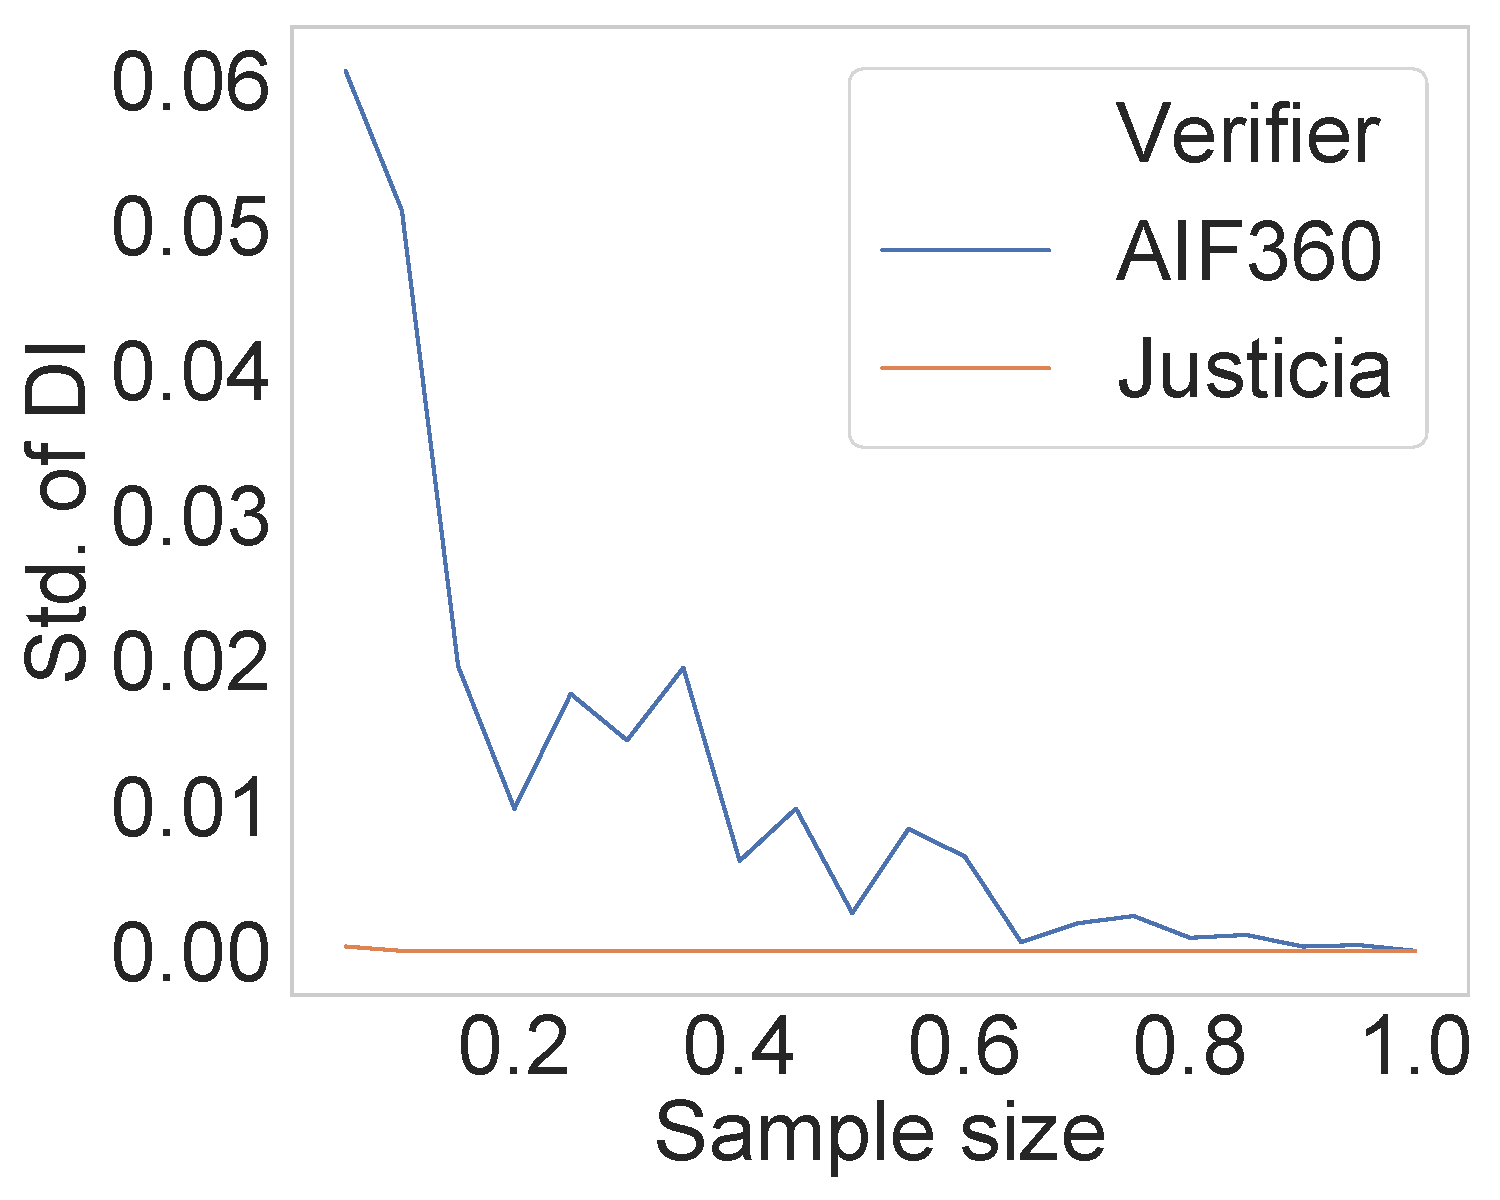
\includegraphics[scale=.2]{figures/fairness/justicia/sampling_DI_after_Adult_rw_LR_race.pdf}}
	\subfloat{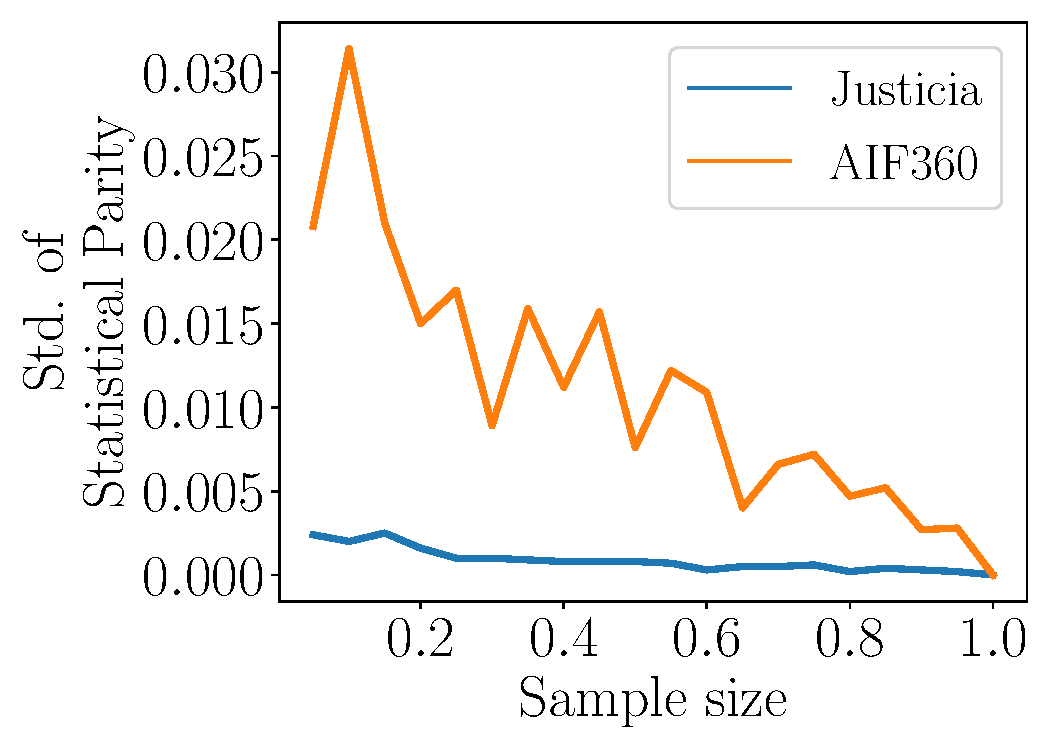
\includegraphics[scale=.2]{figures/fairness/justicia/sampling_SPD_after_Adult_rw_LR_race.pdf}}		
	
	\caption[Robustness of fairness verification]{Standard deviation in estimation of disparate impact (DI) and stat. parity (SP)  for different sample sizes (sample size $ = 1 $ refers to the entire dataset). {\justicia} is more robust with variation of sample size than  AIF360. }
	\label{fairness_justicia_fig:sample-size}
\end{figure*}



\begin{figure}[t!]
	\begin{center}
		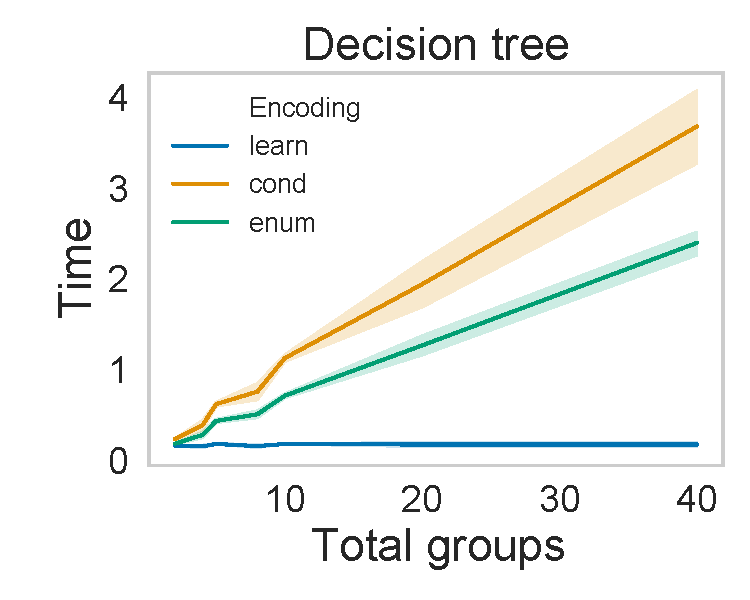
\includegraphics[scale=.4]{figures/fairness/justicia/encoding_runtime_Adult_DT.pdf}
		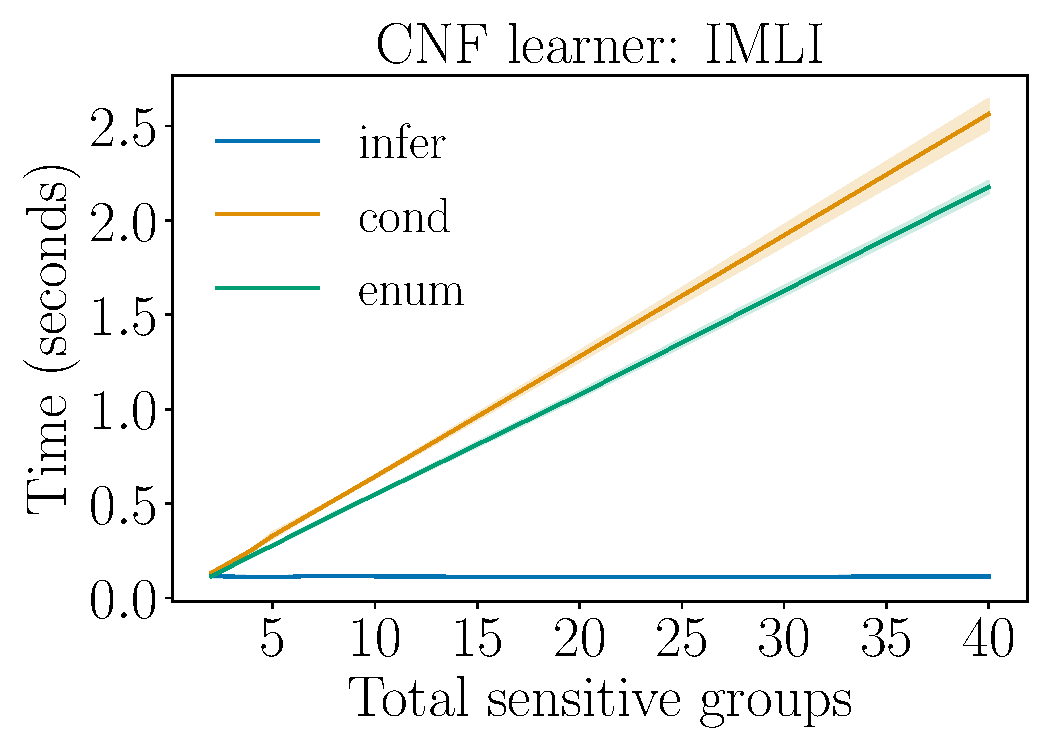
\includegraphics[scale=.4]{figures/fairness/justicia/encoding_runtime_Adult_IMLI.pdf}
		\hfill
		\caption[Runtime of different encodings in {\justicia}]{Runtime comparison of different encodings while varying total sensitive groups in the Adult dataset. \red{Label `learn' to be `infer'???}}
		\label{fairness_justicia_fig:runtime_diff_encodings}
	\end{center}
\end{figure}



\subsubsection{Comparative Evaluation of Different Encodings.}
While both {\justiciaenum} and {\justicialearn}  have the same output according to Lemma~\ref{fairness_justicia_lm:equivalence},  {\justicialearn} encoding  improves exponentially  in runtime  than {\justiciaenum} encoding on both decision tree and Boolean CNF classifiers as we vary the total compound groups in Figure~\ref{fairness_justicia_fig:runtime_diff_encodings}. {\justiciacond} ({\justiciaenum} encoding where we consider conditional probabilities of non-sensitive features w.r.t. sensitive groups) also has an exponential trend in runtime similar to {\justiciaenum}.  This analysis justifies that the na\"ive enumeration-based approach cannot verify large-scale fairness problems containing multiple sensitive features, and {\justicialearn} is a more efficient approach for practical use.

%The runtime efficiency of {\justicialearn} posits it as a more scalable and practical approach to verify fairness than {\justiciaenum}.
%\red{Justify the use of }.








